%*********************第四章******************
\chapter{基于OpenCL的TLD算法高性能实现}
\section{引言}
在前两章中,通过在算法层次上优化当前具有领先精度的跟踪器KCF,以及适用于视觉跟踪的目标候选生成器EdgeBoxes,并将两者有效结合起来,取得了令人满意的视觉跟踪性能。
但是,随着机器视觉应用对精度和鲁棒性的要求不断提高,跟踪器的结构正日趋复杂,计算负载与日俱增,高质量、高性能的跟踪器实现变得越来越关键。
这一点在视觉跟踪领域顶级竞赛VOT(Visual Object Tracking)中也得到了印证。作为第一届VOT竞赛,VOT2013\upcite{vot2013}选取了16个视频序列,每个序列突出一个视觉跟踪中的难点(如遮挡,光照变化等)。首届获胜的跟踪器PLT\upcite{plt}采用二值化特征作为目标描述,并用查找表的方式实现了线性分类器,因此其C++实现达到了169.59 FPS的极高速度。VOT2014\upcite{vot2014}将视频序列扩充为25个,且标记目标物体的矩形框允许旋转,对跟踪器提出了更高难度的挑战。该届获胜的DSST\upcite{dsst}由互相配合的两个相关滤波器构成,一个用于判断目标中心位置,一个用于判断最佳目标大小。结构的简洁性和相关滤波的低计算量使得其Matlab版本也能够做到实时处理(24 FPS)。VOT2015\upcite{vot2015}的视频序列达到了60个,且难度大幅增加。为了应对挑战,MDNet\upcite{mdnet}采用了专门面向视觉跟踪的6层卷积神经网络(CNN),并按照高斯分布大量采样不同位置、不同大小的局部图像进行检测。尽管MDNet在精度和鲁棒性上取得了第一名,但是由于它的计算量很大,实现(Matlab+MatConvNet)又较为粗糙,仅能达到1 FPS的跟踪速度,无法满足实时在线跟踪的要求。

由此可见,在跟踪算法日益复杂的趋势下,为了保证跟踪算法的实用性,或者说为了提高视觉跟踪对计算复杂性的容忍度,研究跟踪算法的高性能实现十分必要。
这里的高性能实现,和``高性能计算''属同一范畴,意指在实现过程中针对硬件体系结构特征,充分发挥计算设备/平台的计算能力。
通过分析体系结构和高性能计算的发展可以看出,并行化无疑是解决高性能实现问题的关键。利用多核并行、向量指令、流水化等并行手段,可以充分发挥通用处理器(CPU)的计算能力。
除了CPU这一经典计算设备,当前包含两类甚至多类计算设备的异构计算平台正方兴未艾。从SoC芯片(如Qualcomm Snapdragon 835\upcite{snapdragon})到嵌入式平台(如Nvidia Jetson\upcite{jetson}),甚至到超级计算机(如天河-1A\upcite{top500}),CPU+GPU的组合已成为一种潮流。要发挥异构平台的计算潜力,除了充分开发算法中的可并行部分以外,
如何同时发挥CPU和GPU的性能,以及如何控制两者间的协作和数据传输等是高性能实现面临的又一挑战。

本章将以TLD\upcite{tld, tldjournal}跟踪算法为例,以OpenCL\upcite{oclspec}作为编程模型,阐述视觉跟踪算法在异构平台下的高性能实现所需的关键技术和面临的问题挑战。严格来讲,TLD算法并非是一个单纯的视觉跟踪算法,而是一个``长时间鲁棒跟踪框架''。它在传统跟踪算法中引入了独立的学习和检测模块,将跟踪-学习-检测三部分有机结合起来:跟踪模块仅根据前一帧判断目标在当前帧中的位置;学习模块构建一个可靠的目标描述,并不断更新它;检测模块在整个帧图像中找出可能包含目标的区域,用以修正跟踪结果。这样的结构,使得TLD比传统跟踪器鲁棒得多,且能适应长时间的目标跟踪。此外,除了TLD本身提供的3个模块算法,各个模块都可以自由替换为具有类似功能的算法,如将跟踪模块替换为KCF跟踪器,将学习模块和检测模块分别替换为RCNN\upcite{fastrcnn, fasterrcnn}的训练过程和检测过程等。因此,研究TLD的高性能实现兼具实用性和理论研究价值,未来应用前景广阔。
另一方面,相比其它并行编程模型如CPU上的OpenMP\upcite{openmp}、GPU上的CUDA\upcite{cudaspec}等,OpenCL是跨平台的,其具备的功能移植性可以使得同一程序(如同一跟踪算法或者同一算法模块)不经修改地在不同异构设备上正确地执行,从而方便地利用异构计算平台下的各种计算设备。因此OpenCL是在异构计算平台下进行高性能跟踪算法实现的一个合适选择。

本章内容安排如下:第2、3节分别介绍OpenCL编程模型和TLD跟踪算法流程;第4节介绍TLD检测模块的第一部分\pozhehao Fern随机森林的高性能实现;第5节介绍检测模块的第二部分\pozhehao 最邻近(Nearest Neighbor,NN)分类器的高性能实现;第6节介绍学习模块中的瓶颈部分的高性能实现;第7节对高性能实现的效果进行评测;最后在第8节进行本章总结。

\section{OpenCL编程模型}
\label{oclmodels}
当前,异构计算平台,即包含了多种异构计算设备(CPU、GPU、DSP等)的计算系统,已经非常普及。用传统方法编写高性能程序已较为困难\pozhehao
面向多核CPU的编程通常使用共享存储模型,主要开发多核间的线程级并行;而面向GPU的编程通常关心复杂的存储层次和数据级并行。
巨大的编程方式差异,导致程序员难以用一种代码来开发多种异构设备的计算能力。

OpenCL(Open Computing Language,开放计算语言) 是一个专门面向异构系统通用目的的编程模型标准。苹果公司于2008年6月首次提出,Khronos工作组于2010年6月正式发布。它的设计初衷就是面向异构计算平台,提供一个统一的编程模型。程序员们只需编写一个程序,就可以方便地利用异构平台的所有计算资源。为了达到这一目的,OpenCL屏蔽了硬件设备的体系结构差异,并用四个抽象模型来描述编程方式和其它细节。

\begin{figure}[htb]
  \centering
  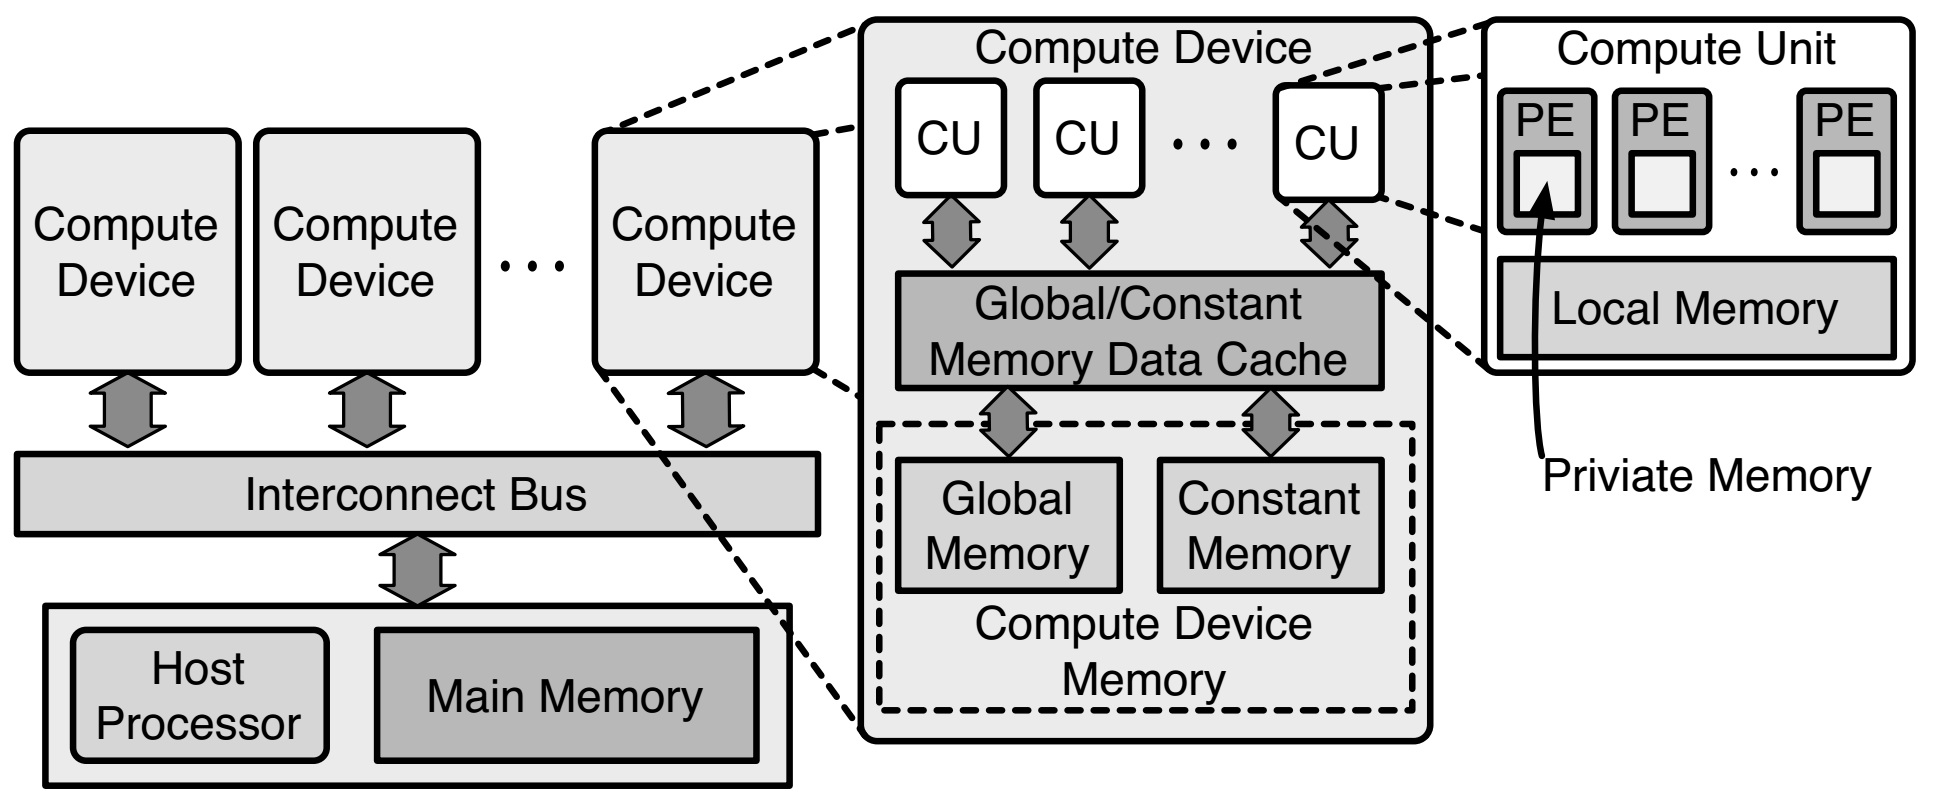
\includegraphics[width=12cm]{ocl_platform_mem_model}
  \caption{OpenCL的平台模型和存储模型\upcite{cell}}
  \label{oclplatformandmem}
\end{figure}

\begin{compactitem}
\item \textbf{平台模型(Platform Model)}
\end{compactitem}

平台模型是OpenCL的抽象低层硬件结构。通过将硬件结构抽象地更为低层,暴露出更多的硬件细节,从而留出更多的编程和优化灵活性;而抽象性又屏蔽了体系结构差异,保证了程序的可移植性。

如图\ref{oclplatformandmem}所示,OpenCL的平台由宿主处理器(Host Processor)和与之互联的一个或者多个计算设备(Compute Device)构成。
每个计算设备又包含一个或者多个计算单元(Compute Unit),而一个计算单元又包含一个或多个处理单元(Processing Element)。
处理单元作为最细粒度的计算承载单位,是一个抽象的标量处理器。

\begin{figure}[htb]
  \centering
  \subfloat[上下文和命令队列\upcite{oclppt}]{%
    \label{comandqueue}
    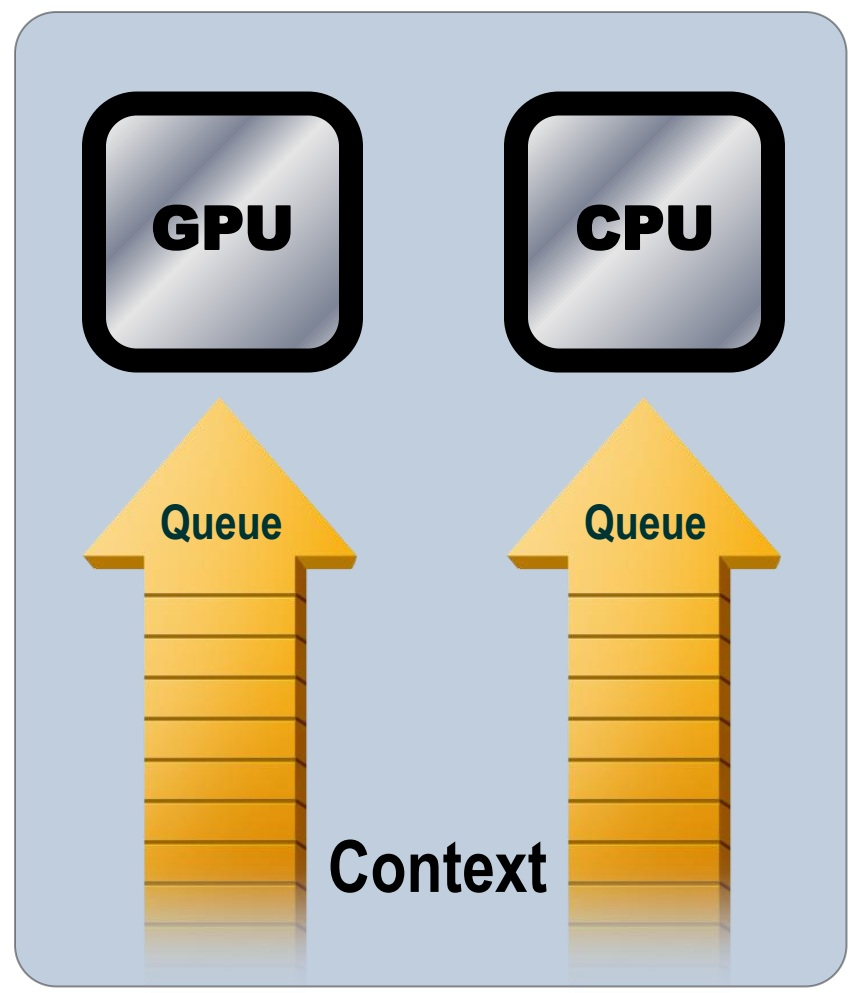
\includegraphics[height=4.5cm]{commandqueue}}\hspace{0.2cm}
  \subfloat[多维索引空间]{
    \label{ndrange}
    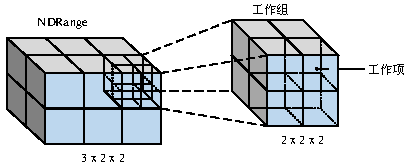
\includegraphics[height=4.2cm]{ndrange}}
  \caption{OpenCL的执行模型}
  \label{oclexecution}
\end{figure}

\begin{compactitem}
\item \textbf{执行模型(Execution Model)}
\end{compactitem}

一个OpenCL程序包括两大部分\pozhehao 宿主程序(Host Program)和Kernel程序(或称内核程序)。

宿主程序用C或者C++编写,运行于宿主处理器之上,通过提交命令(Command)的方式来控制计算设备中的处理单元进行计算,或是控制宿主处理器和计算设备之间的数据传输。
如图\ref{comandqueue}所示,宿主程序会定义一个上下文(Context),上下文中包含了可用的计算设备、待执行的Kernel程序、存储空间等信息。
宿主程序还会为每一个计算设备分配一个或者多个命令队列(Command Queue,或者Queue),并向命令队列中添加命令。随后命令队列就会调度命令进行执行。
命令有三种类型:执行Kernel程序,数据传输,以及同步。

Kernel程序实质上是一个函数,用OpenCL C语言编写,执行于计算设备之上。宿主程序通过提交一个执行Kernel的命令,来启动Kernel程序在计算设备上的执行。
一个Kernel程序有众多的执行实例,对应于一个抽象的多维(一维到三维)索引空间(NDRange Index Space)。
一个Kernel的执行实例对应一个工作项(Work-Item),它是索引空间中的一个最细粒度点,代表着Kernel的一次执行,并根据其在空间中的位置被赋予一个全局索引值(Global ID)。每个工作项都执行相同的Kernel程序,但是由于索引值的不同,各自的执行路径和访问的数据也会不同。
多个相邻工作项组成一个工作组(Work-Group),是对索引空间的更粗粒度分解。根据在索引空间中的位置,工作组也会被赋予一个组索引值(Group ID)。而每个工作组内的工作项,还会根据其组内位置被赋予局部索引值(Local ID)。
OpenCL规定,一个工作组执行于一个计算单元之上,且同一工作组内的工作项是并发执行在计算单元中的处理单元上的。
如图\ref{ndrange}所示,为一个三维的索引空间。该空间包含了$3\times2\times2$个工作组,而每个工作组包含$2\times2\times2$个工作项。

\begin{compactitem}
\item \textbf{存储模型(Memory Model)}
\end{compactitem}

OpenCL的存储模型定义了四个独立的存储空间,分别位于不同的抽象硬件层次之上,且跟执行模型紧密相关。
如图\ref{oclplatformandmem}所示,全局存储(Global Memory)位于计算设备中,任何工作组中的任何工作项都可以读写其中的数据。
常量存储(Constant Memory)是全局存储的一部分,但是其中数据只能被读出而不能被修改。
计算设备还可能提供用以提升全局存储和常量存储性能的高速缓存(Data Cache)。
局部存储(Local Memory)通常位于计算单元之中,仅属于某一个工作组,只能被该工作组中的工作项访问,而对其它工作组来说是不可见的。
私有存储(Private Memory)通常位于处理单元内,是一个工作项所私有的,其它工作项都不可见。

宿主程序可以通过提交数据传输类的命令,来实现宿主处理器的主存(Main Memory)和计算设备的全局存储/常量存储间的数据传输。

\begin{compactitem}
\item \textbf{程序模型(Programming Model)}
\end{compactitem}

这里的程序模型,指的是并行程序的实现方式。OpenCL支持两类并行程序模型,数据并行和任务并行,以及这两类的混合编程。

数据并行是指一个指令序列同时作用于多个存储元素(数据)之上,它是通过定义执行模型中的多维索引空间来实现的。
所有工作项执行相同的Kernel程序,即同一个指令序列;而各个工作项在索引空间中有着不同的索引值,导致根据索引值的访存会访问到不同的数据。
这样一来,同一Kernel程序将同时处理不同数据,实现数据并行。

任务并行是指不同指令序列的同时执行。
实现任务并行,通常是通过在一个或者多个命令队列中,添加多个Kernel执行命令来实现的。


\section{TLD跟踪算法}
\label{sectldalgo}
TLD的命名来自于跟踪(Tracking)-学习(Learning)-检测(Detection)三部分的首字母。
将这三部分有机结合,正是TLD相比于传统跟踪算法的最大区别。
如图\ref{tld}所示,跟踪模块负责计算目标物体在连续两帧间的运动,并提供一个目标候选位置。
它假设目标物体在连续两帧间的运动幅度较小,且目标总是可见的。因此当目标被遮挡或是离开视野时,跟踪模块通常会失效且无法自行恢复。
检测模块将每一帧都看作是独立的,并在整个帧图像中进行搜索检测,从而提供一到多个可能包含目标物体的候选位置。
因此当跟踪模块失效时,检测模块可以重启跟踪。
学习模块会综合考虑跟踪和检测的结果,以最终确定目标物体的位置。
此外,它还会为检测模块提供新的训练数据,以不断提升检测的准确度。

\begin{figure}[htb]
  \centering
  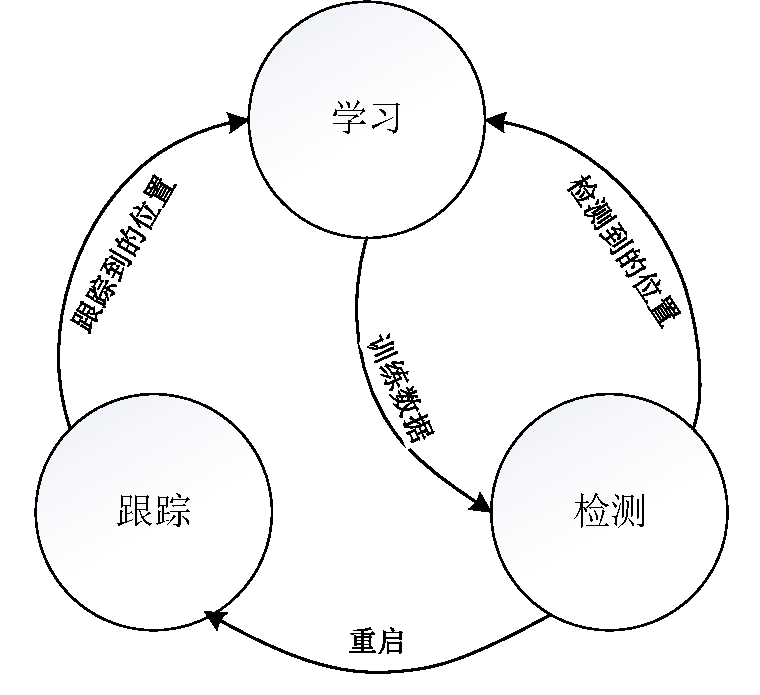
\includegraphics[width=7cm]{tld}
  \caption{TLD跟踪算法的三大部分}
  \label{tld}
\end{figure}

TLD的形式化流程如算法\ref{tldalgo}所示。
更具体地,TLD算法在逐帧运行之前需进行初始化。
初始化的首要任务是构造网格(Grid),即大量的边界框(Bounding Box)。
网格通过用不同的尺度和步长来扫描整幅帧图像得到,与当前帧内容无关,仅与帧大小和目标初始尺度相关。
逐帧运行过程中,检测模块将检测网格中的每一个边界框,找出其中可能包含目标物体的。


\begin{algorithm}[htbp]
  \caption{TLD跟踪算法(对于第$i$帧)}
  \label{tldalgo}
  \algsetup{linenosize=\scriptsize}
  \footnotesize
  \begin{algorithmic}[1]
    \REQUIRE $ $ \\ 当前帧图像$frame[i]$,\\ 前一帧图像$frame[i-1]$,\\ 目标物体在前一帧中的位置(边界框)$lastBB$;
    \ENSURE $ $ \\ 目标物体在当前帧中的位置(边界框)$currentBB$;
    \STATE $trackedBB \leftarrow Tracker( frame[i-1], frame[i], lastBB )$
    \\ $\bullet$ 跟踪模块根据目标物体在前一帧中的位置,计算其在当前帧中的位置,得到$trackedBB$,失效时$trackedBB$为NULL;
    \STATE $detectedBBs \leftarrow Detector( frame[i] )$
    \\ $\bullet$ 检测模块在当前帧中检测出所有可能包含目标物体的边界框,存入$detectedBBs$;
    \STATE $clusteredBBs \leftarrow Cluster( detectedBBs )$
    \\ $\bullet$ 将$detectedBBs$中互相靠近的边界框合并为单个框,存入$clusteredBBs$;
\IF{$trackedBB \neq $ NULL}
    \FOR{\textbf{each} $clusteredBB$ \textbf{in} $clusteredBBs$}
    	\IF{ $Overlap( clusteredBB, trackedBB )  < 0.5$ \AND $NNConf( clusteredBB )  > NNConf( trackedBB )$}
    	\STATE $confidentBBs \leftarrow clusteredBB$ 
    	\ENDIF
    \ENDFOR
    \\ $\bullet$ 从$clusteredBBs$中选出距离$trackedBB$较远,但是置信度更高的边界框,存入$confidentBBs$;
    \IF{ $Sizeof( confidentBBs ) = 1$ }
    \STATE $currentBB \leftarrow confidentBBs[0]$ 
    \\ $\bullet$ 如果$confidentBB$是唯一的,则认为跟踪模块出错,重启跟踪模块;
	\ELSE 
	\STATE $currentBB \leftarrow WeightedAverage( trackedBB, detectedBBs )$ 
	\\ $\bullet$ 否则,以$trackedBB$为主,将$trackedBB$和它附近的$detectedBBs$进行加权平均,得到当前目标位置;
    \ENDIF
    \\ $\bullet$ 跟踪模块有效时,$trackedBB$和$detectedBBs$共同决定$currentBB$;
\ELSE
	\IF{ $Sizeof( clusteredBBs )  = 1$ }
	\STATE $currentBB \leftarrow clusteredBBs[0]$
	\ENDIF
	\\ $\bullet$ 跟踪模块失效时,若存在唯一的$clusteredBB$,则用它来重启跟踪模块;
\ENDIF

	\IF{ $trackedBB \neq $ NULL \AND $Validated( trackedBB ) $ }
    \STATE $ Learn( currentBB, frame[i] )  $
    \ENDIF
    \\ $\bullet$ 若$trackedBB$通过验证,则学习模块根据$currentBB$提取正负样本,训练检测模块。
  \end{algorithmic}
\end{algorithm}

函数$Tracker()$的主要部分是LK(Lucas-Kanade)光流跟踪\upcite{lkoptflow, lkoptflow2},属于跟踪模块。
LK光流跟踪算法会运行两次,第一次用于估计目标物体从$frame[i-1]$到$frame[i]$的运动;第二次逆向运行,根据估计到的$frame[i]$中位置,
计算物体在$frame[i-1]$中的原位置。
通过对比$lastBB$和两次LK光流计算的结果,可以判断出LK光流跟踪是否成功,即跟踪模块是否有效。
%如果LK光流跟踪成功,还需利用最邻近分类计算其结果位置的置信度($NNConf()$)。

%只有置信度高于阈值时,跟踪模块才有效,$Tracker()$才会输出$trackedBB$。

函数$Detector()$主要包括两部分,Fern随机森林\upcite{fern}分类和最邻近分类(Nearest Neighbor Classifier),均属于检测模块。
首先,Fern随机森林将作用于网格中的大量边界框,并得出响应值。该响应值反映了边界框恰好包围目标物体的概率。
随后,响应值高于阈值的边界框将通过最邻近分类,计算出置信度($NNConf()$)。
最邻近分类的模型为一组正负样本图像块,置信度的计算过程为将输入图像块与正负样本逐一进行相似度对比。
这里的相似度使用NCC(Normalized Cross-Correlation,归一化互相关)\upcite{ncc}来度量,
而置信度由输入图像块与正样本的相似程度,以及它与负样本的不相似程度共同决定。
置信度高于阈值的边界框才能作为$Detector()$的输出。
函数$Cluster()$将$Detector()$输出的边界框进行聚类,把互相靠得太近的多个边界框合并为一个,以进一步减少数目。

目标物体在当前帧中的位置最终由学习模块来确定。如果跟踪模块有效,则综合考虑跟踪和检测的结果:
若$clusteredBBs$中存在且仅存在一个置信度高于$trackedBB$的边界框,则认为跟踪模块出错,用检测结果替代跟踪结果;
否则,将跟踪结果与它附近的检测结果进行加权平均,作为最终目标位置。
如果跟踪模块失效,未避免歧义,当且仅当$clusteredBBs$中有唯一边界框时,用来作为最终目标位置。

学习模块还负责决定进行学习的时机,即跟踪结果足够可靠时\pozhehao 跟踪模块有效,且$trackedBB$通过了验证。
$Validated()$函数在两种情况下认为验证通过:$trackedBB$经过最邻近分类得到的置信度足够高;或者在某一历史帧中置信度足够高,
且从那时起跟踪模块从未失效或出错。
学习过程$Learn()$分为两步,提取正负样本和再训练检测模块。
提取正负样本前,需要先计算网格中所有边界框与$currentBB$的重叠率($Overlap()$)。
对于Fern随机森林,选取重叠率低且响应值较高的边界框作为负样本,即``难反例挖掘(Hard Negative Minning)'';
同时选取重叠率高的边界框,并进行随机旋转缩放,作为正样本。
对于最邻近分类器,从$detectedBBs$中选取重叠率低于阈值的边界框作为负样本;
同时以重叠率最高的边界框作为唯一正样本。
再训练Fern随机森林的过程,即是更新每一棵随机树的叶节点权值的过程。通过记录落入每一个叶节点的正负样本总数,更新其权值。
再训练最邻近分类器的过程,即是验证正负样本是否与当前模型冲突(正样本的置信度太低,或负样本置信度太高)的过程。
将冲突的正负样本加入模型中就完成了更新。

通过测试TLD算法的官方串行版本OpenTLD\upcite{opentld},以及借鉴H-TLD\upcite{htld}中的性能分析,
同时考虑到OpenCL会带来的额外开销,本章将以OpenTLD为基础,对其中的计算密集部分和性能瓶颈部分用OpenCL进行高性能实现。
这些部分包括Fern随机森林分类,最邻近分类,学习过程中的重叠率计算、正负样本提取。
LK光流跟踪部分也是计算密集的,但由于OpenTLD所依赖的OpenCV\upcite{opencv}库已提供了OpenCL版本的实现,因此这里不再重复实现。
至于其它部分,有的计算量太小(如确定最终目标位置时,$clusteredBBs$中边界框数量通常很少),有的不适于用OpenCL并行化(如再训练过程中,分支过于密集)。

\section{Fern随机森林的高性能实现}
在进行Fern随机森林分类之前,OpenTLD先对网格中的所有边界框进行一次方差过滤,以减少输入随机森林的边界框数量。
边界框对应的图像块的灰度值方差被计算出来,若该方差低于初始帧中目标物图像块的方差,那么该边界框将被过滤掉。
虽然网格中边界框很多,但由于采用了``积分图(Integral Image)''方法,方差过滤十分高效,计算量较小。

如\ref{sectldalgo}节所述,即使加入了过滤步骤,Fern随机森林仍将作用于大量边界框,因此必须十分高效。
TLD算法中,用于分类的特征是基于``像素对比''生成的,即根据边界框提取出图像块,然后在图像块中按照预定模式采样13对像素点,并进行灰度值对比。如果用$0$和$1$来表示对比结果,则13对像素点的对比结果可用一个二进制向量表示,即Fern特征向量。
上述过程被称作特征提取,如图\ref{fernfig}中的``特征提取''部分所示。

\begin{figure}[htb]
  \centering
  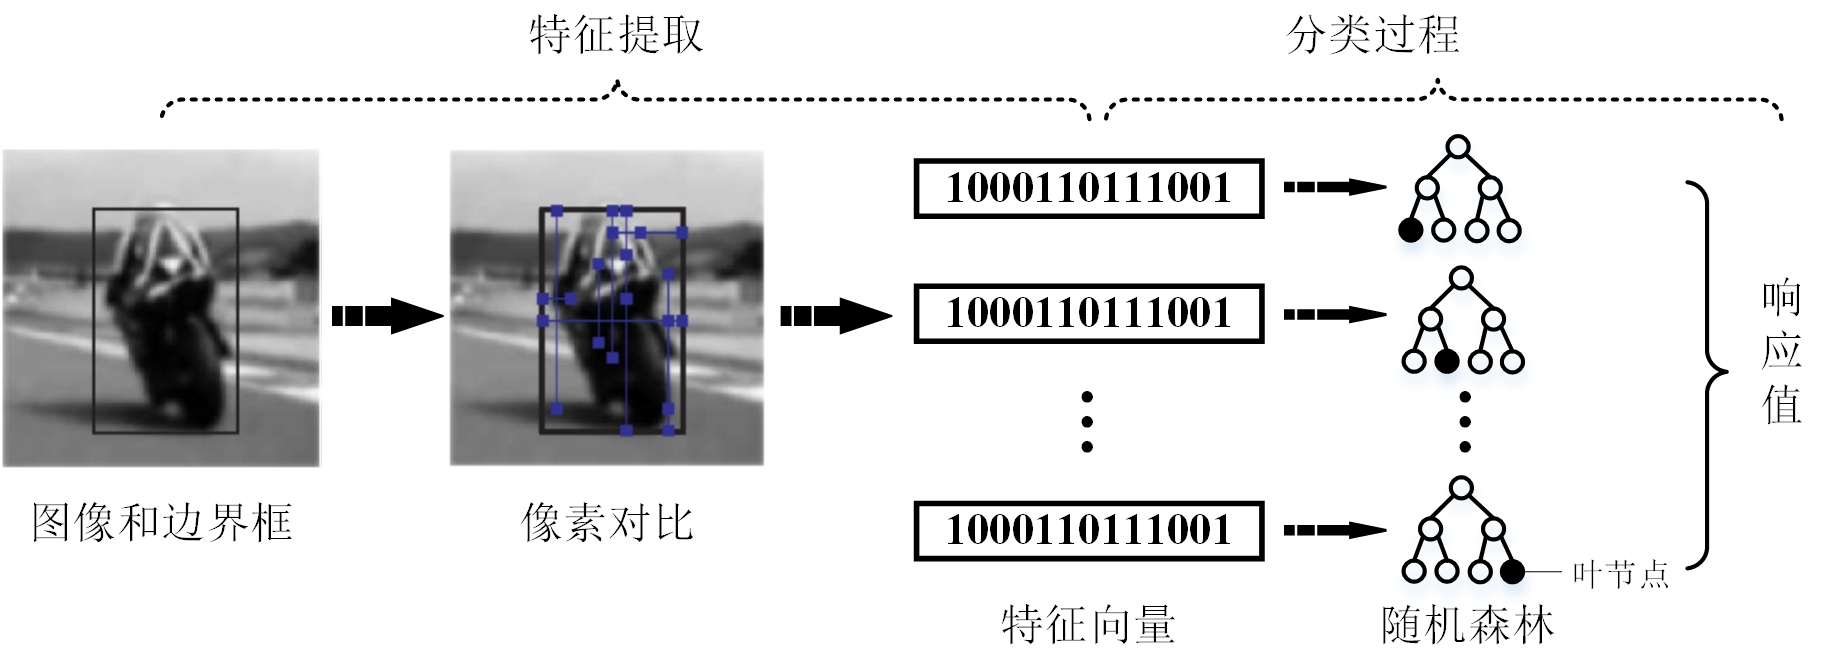
\includegraphics[width=13cm]{fernfig}
  \caption{Fern随机森林分类的流程}
  \label{fernfig}
\end{figure}

由于网格中的边界框有着不同的尺度大小,TLD为每一个尺度定义了10种采样像素点对的模式,每一种采样模式都定义了13个点对的不同采样位置。
因此,每一个边界框通过特征提取后都会得到10个13位的Fern特征向量。
为了对这些特征向量进行分类,TLD针对每一种采样模式(即每一个Fern特征向量)构造一棵随机树,总共10棵随机树构成了Fern随机森林。
随机树的叶节点被赋予权值,代表着边界框包含目标物体的概率。
每个Fern特征向量经过对应随机树的分类后,都会落入该随机树的一个叶节点中。
将10个随机树叶节点的权值进行平均,即得到Fern随机森林的响应值。
上述过程即是Fern随机森林的分类过程,如图\ref{fernfig}中的``分类过程''部分所示。

\subsection{特征提取的并行化}
Fern随机森林特征提取的输入为当前帧图像、网格、候选边界框索引、以及像素点对采样模式;输出为所有候选边界框对应的Fern特征向量。
%在利用OpenCL进行特征提取前,需要对输入数据进行重构。
在本章的高性能实现中,帧图像的灰度值被存储在一个一维数组中。
网格在初始化时就构造好了,为一个一维数组,每5个元素代表一个边界框,分别是$\{x, y, width, height, scale\_id\}$,即左上角横、纵坐标、宽、高和尺度索引。
因为网格数组在整个跟踪过程中不会变动,因此将它放入OpenCL的常量存储中,供多个Kernel使用,而无需每次都进行分配和释放。
候选边界框索引是方差过滤步骤的输出,为一维数组,每个元素都代表着一个候选边界框在网格数组中的位置。




\subsection{分类过程的并行化}
\subsection{与跟踪器重叠执行}

\section{最邻近分类器的高性能实现}
\subsection{算法流程}
\subsection{分类过程的并行化}

\section{学习过程的高性能实现}
TLD学习过程的流程
\subsection{重叠率计算和负样本提取的并行化}
\subsection{正样本提取的并行化}

\section{实验评测与分析}
\subsection{Kernel性能评测与分析}
在CPU、GPU上,纯Kernel的执行时间;性能移植性问题

算上数据重组、传输等额外开销的执行时间

\subsection{整体性能评测与分析}
全部Kernel在CPU上执行;全部Kernel在GPU上执行(可重叠);各Kernel在适合的设备上执行(最优性能)

\section{小结}